%%%%%%%%%%%%%%%%%%%%%%%%%%%%%%%%%%%%%%%%%%%%%%%%%%%%%%%%%%%%%%%%%%%%%%%%%%%%%%%%
%2345678901234567890123456789012345678901234567890123456789012345678901234567890
%        1         2         3         4         5         6         7         8



\documentclass[letterpaper, 10 pt, conference]{ieeeconf}  % Comment this line out if you need a4paper

%\documentclass[a4paper, 10pt, conference]{ieeeconf}      % Use this line for a4 paper

\IEEEoverridecommandlockouts                              % This command is only needed if 
                                                          % you want to use the \thanks command

\overrideIEEEmargins                                      % Needed to meet printer requirements.

%In case you encounter the following error:
%Error 1010 The PDF file may be corrupt (unable to open PDF file) OR
%Error 1000 An error occurred while parsing a contents stream. Unable to analyze the PDF file.
%This is a known problem with pdfLaTeX conversion filter. The file cannot be opened with acrobat reader
%Please use one of the alternatives below to circumvent this error by uncommenting one or the other
%\pdfobjcompresslevel=0
%\pdfminorversion=4

% See the \addtolength command later in the file to balance the column lengths
% on the last page of the document

% The following packages can be found on http:\\www.ctan.org
\usepackage{graphicx} % for pdf, bitmapped graphics files
\usepackage{epsfig} % for postscript graphics files
\usepackage{mathptmx} % assumes new font selection scheme installed
\usepackage{times} % assumes new font selection scheme installed
\usepackage{amsmath} % assumes amsmath package installed
\usepackage{amssymb}  % assumes amsmath package installed
\usepackage{stackengine}
\usepackage{booktabs}
\usepackage{physics}
\usepackage{comment}
\usepackage{wrapfig}
\usepackage{tcolorbox}
\usepackage{tikz}
\usepackage{pgfplots}
\pgfplotsset{ticks=none}
\usepackage{multirow}
\usepackage{amsmath,amssymb,amsfonts}
\usetikzlibrary{calc}
\usetikzlibrary{arrows}
\usetikzlibrary{patterns}
\usepackage{bondgraphs}
\usetikzlibrary{shapes,positioning, fit, backgrounds}
\usepackage{commath}
\usetikzlibrary{intersections}
\usetikzlibrary{arrows,shapes,   calc, patterns,decorations.pathmorphing,decorations.markings}
\tikzset{
block/.style = {draw, fill=white, rounded corners, minimum height=1em, minimum width=1em},
tmp/.style  = {coordinate}, 
sum/.style= {draw, fill=white, circle, node distance=1cm},
input/.style = {coordinate},
output/.style= {coordinate},
container/.style = {draw, rounded corners,
                     inner xsep=2mm, inner ysep=2mm},
pinstyle/.style = {pin edge={to-,thin,black}
}
}


\def\delfy{\mathrel{\ensurestackMath{\stackon[1pt]{=}{\scriptstyle\Delta}}}}
\newtheorem{theorem}{Theorem}[section]
\newtheorem{lemma}{Lemma}[section]
\newtheorem{proposition}{Proposition} [section]                            % Theorem head font

\title{\LARGE \bf 
A Bond Graph modeling perspective to price dynamics in the global oil-economic system}


\author{
		Coen Hutters, Nicolaas Orie, Max Mendel 
% 
\thanks{
C.~Hutters and M.~Mendel are with the Delft Center for Systems and Control, Delft University of Technology, Mekelweg 2, 2628 CD, Delft, The Netherlands. 
{\tt\small \{c.hutters-1, m.mendel\}@tudelft.nl}
%
}
}



\begin{document}



\maketitle
\thispagestyle{empty}
\pagestyle{empty}


%%%%%%%%%%%%%%%%%%%%%%%%%%%%%%%%%%%%%%%%%%%%%%%%%%%%%%%%%%%%%%%%%%%%%%%%%%%%%%%%
\begin{abstract}
 

\end{abstract}


%%%%%%%%%%%%%%%%%%%%%%%%%%%%%%%%%%%%%%%%%%%%%%%%%%%%%%%%%%%%%%%%%%%%%%%%%%%%%%%%

\section{Introduction}
\label{sec: intro}




The global energy system is undergoing a mayor shift. Carbon-based energy carriers, such as crude oil and natural gas, are being partly replaced by electrification alternatives such as electricity storage and hydrogen. [Global Energy and Climate Outlook 2019: Electrification for the low-carbon transition]. 
This shift to a hybrid and more complex energy system calls for new energy models that are capable of dealing with complexity, non-equilibrium conditions and uncertainty. [Emergence of New Economics Energy Transition Models: A Review].

 
Current modelling techniques to model oil-economic systems can be subdivided in three categories; structural, computational, and reduced form (econometric models) [Hillard G. Huntington. Oil markets and price movements: A survey of models. SSRN Electronic Journal, May 2003.]. Structural models are first-principle, agent-based systems models. Structural models lack the ability to yield quantitatively reliable results. 
Computational models are first-principle equilibrium models of economic systems.
These models yield reliable quantitative results, but lack the ability to model non-equilibrium systems. 
Reduced form (econometric) models are regression models on time-series data.
These models can accurately model short-term variability, but are not able to make predictions outside the variable space on which these models are trained.
This inability is a crucial shortcoming of regression models given the shifting energy system.

In this paper, we introduce the use of dynamical systems theory to model the oil market.
In particular, we use the bond graph modelling method to derive a first-principles model of the price and inventory dynamics in the oil market.



Bond graphs are graphical tools used to model dynamical systems \cite{}.
The bond graph method was introduced by Henry Paynter who noted that the dynamics of engineering systems from different domains, e.g. electrical, mechanical, or hydraulic engineering, were described by differential equations of the same form.
In a bond graph, elements are interconnected by power bonds that represent the time rate of energy flow between the elements as the product of \textit{flow} and \textit{effort} variables.
Furthermore, each power bond indicates the causality at each element port, i.e. whether an element is driven by a {flow} variable, or its dual {effort} variable. 
The assignment of causality throughout a system must follow structured rules, leaving no room for ambiguous causal relations.
Bond graph theory has been extended to mechatronics, thermodynamics, hybrid and switching systems, and even social and economic systems.

The extension to economic systems was first introduced by Brewer.
Brewer's analogy has been further used in a port-Hamiltonian formulation of macroeconomic systems in ?? and in a macroeconomic bond graph including fractional-order elements in machado.
In Brewer's analogy, money is the economic analog of energy.
As a result of this choice, power bonds represent the cash flow between elements where cash flow is the product of price, the effort variable, and commodity flow, the flow variable.
This however entails that, besides inventory stock, the state variable is the time-integral of price, which Brewer refers to as the \textit{economic impulse}.
Using this analogy it is therefore not possible to derive a first-principles model of the price dynamics of an economic process.

In this paper we introduce an alternative economic bond graph analog in which cash flow, or income, is the economic analog of energy.
Economic bond graph elements are then linked by bonds that represent the exchange of growth.
Here, growth is the product of price movement and commodity flow, representing the economic effort and flow variables, respectively.
In this analogy, bond graph models can be used to model the dynamics of inventory stocks and of prices.



















\begin{comment}
In dynamical systems theory, the time evolution of the system is derived from its current state.
For example, the time evolution of mechanical system can be derived from its current state variables through Newton's equations of motion and that of an electrical system through Maxwell's equations.
For the time evolution of commodity markets, we will use an analogy between engineering and economic systems that results in the equations of motion of economic processes.
This economic-engineering analogy has been developed by the <third> author of this paper and will be presented in detail in future work.
In the present section, we introduce the concepts from the economic-engineering analogy that are relevant for the contribution made in this paper.
We first introduce the description of a commodity market as a dynamical system and then introduce the analogy between mechanical elements and economic phenomena.
\end{comment}




\section{Bond graph modeling of dynamical systems}
Bond graphs describe systems as the interconnection of subsystems, or elements.
Each element has a $port$ through which it can be connected to its environment.
The ports of elements are interconnected by bonds that represent the bi-directional flow of two power variables, effort and flow.
The product of the effort and flow determines the rate of energy exchange between elements per unit of time, i.e. the power.
Power and energy are domain neutral phenomena.
Effort and flow are the generalized description of the signals that make up power in specific engineering domains.
For example, in mechanical systems power is the product of force (effort) and velocity (flow) and in electrical systems power is the product of voltage (effort) and current (flow).
For this reason, force and velocity are said to be the \textit{analog} of voltage and current, respectively.\footnote{In alternative, equally valid analogy voltage is the analog of velocity.\cite{}.}

The basic bond graph elements are divided into 1-port, 2-port, and multi-port elements.
The 1-port elements are the inertia, the capacitor, the resistor, and the active effort source and flow source.
Each 1-port element has a constitutive relation that relates the two power variables.
In case of the inertia and the capacitor this relation includes a time integral that keeps track of a stored state variable. 
The constitutive relation of a inertia is $f= \phi_I^{-1}(p)$, where $p=\int e dt$ and a capacitor is $e = \phi_C (q),$ where $q =\int f dt$,
The dynamics of the state variables are defined by the entire bond graph model.
This time integral also implies a preferred causality, i.e. a preferred effort or flow input.
The resistor dissipates energy and does not have a preferred causality; its causality depends on how it is interconnected to the rest of the system.
A resistor may return an effort for a flow input, $e=\phi_R(f)$, or return a flow for an effort input, $e=\phi_R^{-1}(e)$.
The 2-port elements are the transformer and gyrator.
A transformer links one effort $e_1$ to another effort $e_2$ and one flow $f_1$ to another flow $f_2$ in a power-preserving manner, i.e. $e_1f_1=e_2f_2$.
The gyrator links one effort $e_1$ to a flow $f_2$ and vice versa, again in a power-preserving manner.
The multi-port elements are the 0-junction and the 1-junction.
The multi-port elements represent the interconnection structure between elements. 
The 0-junction is an interconnection structure in which the flow variables sum up to zero and the effort variable is common,$f_1+\dots+f_n=0$, $e_1=\dots =e_n$ , e.g. an electrical node.
In the interconnection structure of the 1-junction the effort variables sum up to zero and the flow variable is common, $e_1+\dots+e_n=0$, $f_1=\dots =f_n$, e.g. an electrical loop.

\begin{tcolorbox}
make tables.
\end{tcolorbox}

\subsection{Bond graphs for economics}
Brewer extended the bond graph analogy in \cite{} by choosing the rate of orders as flow variable and the unit commodity price as effort variable.
The motivation behind this choice is that the power conservation at junctions,
\begin{equation*}
    e_1f_1+e_2f_2+\dots e_nf_n=0,
\end{equation*}
represents Walras' law for proper cash accounting.

However, choosing price as an effort variable entails that the time-integral of price, which Brewer calls the \textit{economic impulse}, is the economic generalized momentum.




This choice of variables, in particular the choice of price as an effort variable excludes the possibility of deriving price dynamics.

We propose to view price not as an effort variable, but as a generalized momentum.
This implies that the effort becomes a signal that provokes a rate of price movement, analogous to how a force provokes a rate of change in momentum.
In general, we refer to the economic effort variable as a \textit{desirability}.

Using this analogy, the power conservation at junctions represents the conservation of growth in an economic system. 

\section{Bond Graph representation of oil-market dynamics}
\label{sec: EconEng}

\subsection{crude oil price drivers}
The oil-economic literature identifies multiple factors that affect the price of crude oil.
The US Energy Information Administration (EIA) captures the four most important factors in a simple model, shown in Figure \ref{fig:EIAmodel}.
The four factors consist of supply, demand, inventory balance, and the financial markets.
An extensive analysis of the EIA model supported by a literature review is provided in \cite{Lang2020}.
In this section, we discuss how the four factors can be modeled with dynamical systems theory resulting in a dynamical systems model for oil prices.




\subsection{Oil Price as dynamical state}
We consider the oil price as a dynamical state.
The oil price changes over time due to the effect of supply, demand, inventories, and financial markets.
We model this by the following dynamical law
\begin{equation}
\label{eq: pdot}
    {p}(t) = \int F(t) dt,
\end{equation}
where $p(t)$ is  the oil price in $\$/\#$ and $F(t)$ is an ''economic force'' applied by on or more factors in $\$/\#\cdot$ yr.
We introduce the specific economic force of each factor in the rest of this section.

The notion of price as a dynamical state is analogous to the notion of inventory, or stock, as a dynamical state.
Inventory dynamics follow the physical law
\begin{equation}
    \label{eq: qdot}
 q(t) = \int Q (t) dt,
\end{equation}
where $Q(t)$ is the net flow of assets in $\#/$yr.


\subsection{Competitive and OPEC Oil supply}
Oil supply is identified as a driver of the long-term equilibrium price.
Oil supply is typically divided in Organization of the Petroleum Exporting Countries (OPEC) and non-OPEC production.
This division is made because the OPEC members produce with respect to a central coordination and are mostly in hands of national oil companies, whereas non-OPEC producers are mostly in hands of investor-owned companies that make independent decisions.

To make the same distinction between OPEC and non-OPEC members, we will model non-OPEC members as inductive elements and OPEC members as controlled current sources.

\subsubsection{non-OPEC members}
Non-OPEC oil producers make independent decisions.
In addition, they are assumed to make decisions so as to make return on investments at the actual market price.


We model each non-OPEC producer as a cost-minimizing agent, i.e. ignoring investments.
Each producer $i\in I$ controls a production path $\gamma_i$ for the upcoming period $T_p$.  
The $i^{\text{th}}$ producer's problem is 
\begin{equation}
    \label{eq: prod}
\begin{split}
\min_{\gamma_i} &\int_{0}^{T_p} L_{i}({y}_i)  \dif \tau \\
&\text{s.t.}\ {y}_i \in Y_i 
\end{split}
\end{equation}
Here, $Y_i$ is the set of achievable production levels of producer $i$. 
We assume that the running cost $L_{i}$ takes the following form
\begin{equation}
\label{eq: Li}
\begin{split}
 L_{i}=     \underbrace{\frac{1}{2}{{y}_i(t)}^TE_{i}^{-1}{{y}_i(t)}}_{\text{variable cost}}+\underbrace{{p}_{f,i}(t )^T{{y}_i}(t )}_{\text{fixed cost}}- \underbrace{ \lambda(t)^T{{y}_i}(t )}_{\text{revenue}},
 \end{split}
\end{equation}
where $y_i \in \mathbb{R}^1$ is the production, $E_i$ is the price elasticity of supply of the $i^{th}$ producer, $p_{f,i}$ are the fixed costs, and $\lambda$ is the market price.   

After applying the calculus of variations the optimization problem (\ref{eq: prod}) results in the affine supply function
\begin{equation}
y_i(t) = \begin{cases}
E_i(\lambda(t)-p_{f,i}) & \text{if}\ \lambda\geq p_{f,i}\ \text{and}\ y_i(t) \in Y_i\\
0 & \text{if} \lambda\leq p_{f,i}
\end{cases}
\end{equation}

\begin{figure}
    \centering
    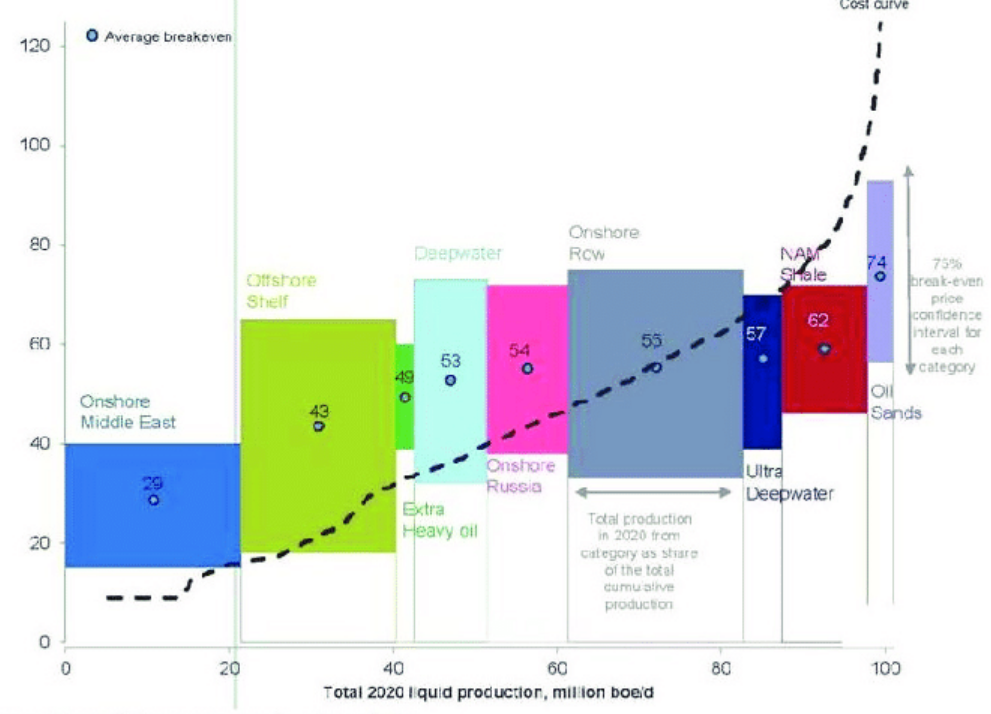
\includegraphics[width=.4\textwidth]{Figures/cost curve.PNG}
    \caption{Marginal cost curve of crude oil as piecewise-affine function}
    \label{fig:marginalcost}
\end{figure}

\subsubsection{OPEC}
OPEC members do not produce according to a free market principle, i.e. basing production levels on the market price.
Instead, the organization sets predetermined production targets for its member countries.
The cost-minimization model used for non-OPEC members thus does not apply to OPEC members.

In this paper, we consider the supply from OPEC members as an external disturbance.

\begin{equation}
    Q(t) = d(t)
\end{equation}

In the discussion section we propose objective functions that may predict the oil supply from OPEC members.


\subsection{Oil demand}
On the demand side, the EIA model makes a distinction between member states of the Organization of Economic Cooperation and Development (OECD) and non-OECD countries.
Most developed countries, e.g. the US and countries in the European Union, are members of the OECD.
The oil consumption in OECD countries is less dependent on economic growth than for developing countries.
This is because the GDP of developed countries is more stable, tax policies slow down oil consumption, and developed countries have larger service industries relative to manufacturing industries.
As a result, the oil consumption in OECD countries is mostly dependent on the oil price.

We model each OECD consumer similar to how we model non-OPEC producers.
This entails that each consumer $j\in J$ controls its consumption path .....


....


Many non-OECD members are developing countries, among which China, India, and Saudi Arabia are the biggest consumers.
In non-OECD counries, oil consumption is stronger related to economic growth rather than to oil prices.
This is a result of on the one hand changing conditions in developing economies, such as increases in population and purchasing power, and on the other hand the higher share of manufacturing industry and use of oil as energy source and feedstock.   
Therefore, non-OECD consumption cannot be modeled like OECD consumption.
Instead, we propose to model non-OECD consumption as an external disturbance that varies with the economic growth of these countries.

Some non-OECD countries control domestic oil prices, preventing consumers to react to global oil price changes.
In the discussion section we propose a model of these countries as disturbance-rejecting controller.





\subsection{Inventories}
The difference between supply and demand is stored in inventory.
The inventory level is a state variable $q$.
The inventory level changes over time by the kinematic relation
\begin{equation}
    \dot{q} = Q_S-Q_D,
\end{equation}
where $Q_S$ is the oil supply, and $Q_D$ is the oil demand.
In case $Q_S>Q_D$, inventory levels rise, and in case $Q_D>Q_S$ inventory levels decrease.
A positive-valued inventory level $q(t)$ indicates a long position of oil that is physically stored, whereas a negative $q(t)$ indicates a short position registered in order books.

We model the convenience of having an inventory as an economic force that is proportional to the inventory level:
\begin{equation}
    F_C(t) = -k (q(t)-q^*),
\end{equation}
where $F_C$ is the convenience ''force'', $k$ is a constant indicating the elasticity of the storage, and $q^*$ is a desired inventory level.
The convenience equation implies that there is a positive (negative) force that drives the price of oil up (down) when the inventory level is below (above) the desired level. 

The oil inventories act as buffer between supply and demand.
When supply exceeds demand, oil can be stored in inventory, and when demand exceeds supply oil may be extracted from the inventories.
We recognize this principle as the analog of a capacitor in an electric circuit that may charge or discharge in case of alternating currents, or as the analog of a spring that can integrate the difference between two velocities.
As the capacitor or spring, oil inventories do not only play a role in the kinematics of the system, i.e. describing the current, velocity, and flow of oil, respectively, but also in the dynamics describing the voltages, forces, and economic forces, respectively.





\subsection{Financial markets}
Multiple activities on the financial markets influence the price of oil.
Oil future contracts, commodity exchange contracts, others.
Some are complex. 

In the model presented in this paper, we only consider the effect of oil traders.

\begin{equation}
    F_T = c (Q_D - Q_S),
\end{equation}
where $c$ is a discounting constant.

In the discussion section, we propose how futures contracts may be modeled in the economic-engineering framework.

We omit the 
\section{Dynamical Systems Model of the Oil Economy}
\label{sec: model}

\begin{figure}
    \centering
    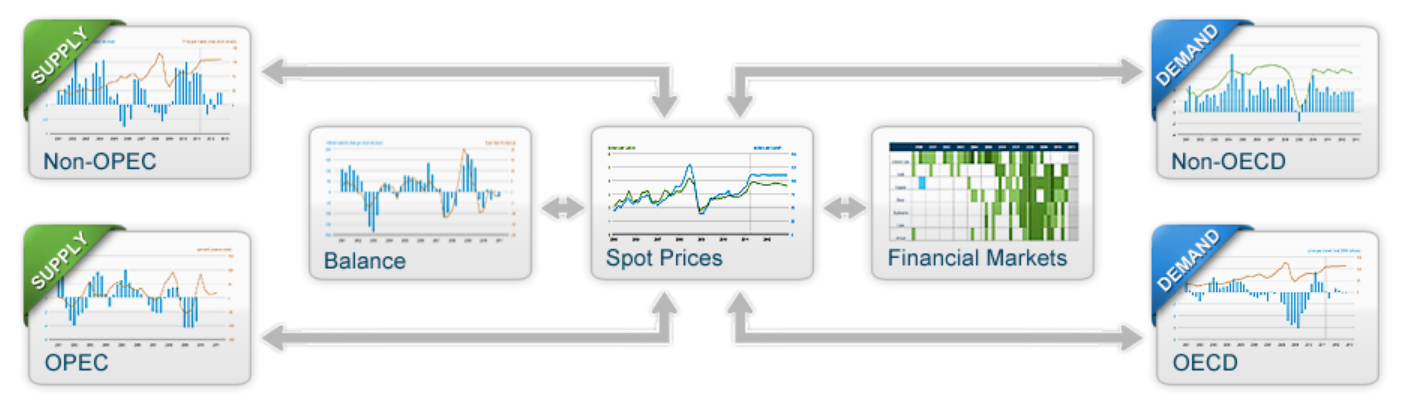
\includegraphics[width=.5\textwidth]{Figures/oilmarketscheme.PNG}
    \caption{Schematic view of what drives oil prices [eia].}
    \label{fig:EIAmodel}
\end{figure}



\subsection{Model Assumptions} 
\begin{itemize}
    \item Inelastic, unknown OPEC Supply
    \item Elastic non-OPEC Supply
    \item Ignore Lead Time
    \item All oil is fungible
    \item Linear aggregation producers
    \item Linear aggregation consumers
    \item market price equals competitive production cost
    \item Ignore Futures Market
    \item Ignore Economic Growth (pre filtered)
    \item Ignore capacity constraints
\end{itemize}

\begin{figure}
    \centering
\begin{tikzpicture}[every node/.style={bgelement},every edge/.append style={bond}]
\node at (0,0) (0junc) {0};
\node at (0,1) (up) {};
\node[label=left:$non-OPEC$,left=1 of up] (nOPEC) {I};
\node[label=right:$non-OECD$,right=1 of up] (nOECD) {$\textbf{S}_f$};
\node[label=right:$OECD$,below=1 of nOECD] (OECD) {I};
\node[label=left:$OPEC$,below=1 of nOPEC] (OPEC) {$\textbf{S}_f$};
\node[label=below:$e$,below=1 of 0junc] (1junc) {1};
\node[label=left:$Balance$,left=1 of 1junc] (C) {C};
\node[label=right:$Fin.\ markets$,right=1 of 1junc] (R) {R};
\draw
(0junc) edge[e_out] (nOECD)
(0junc) edge[e_out] (OECD)
(OPEC) edge[e_in] (0junc)
(nOPEC) edge[e_in] (0junc)
(1junc) edge[e_out] (0junc)
(C) edge[e_out]  (1junc)
(R) edge[e_out]  (1junc)
\end{tikzpicture}
\caption{Bondgraph model of Oil market based on the EIA model.}
    \label{fig:bondgraph}
\end{figure}

Figure \ref{fig:bondgraph} shows an engineering bondgraph model that is analogous to the EIA oil model.
Each bond represents a transmission of oil and of economic force between the connected element and its environment. 
The direction of the flow of oil is opposite to the direction of the economic force.
The so-called causal stroke at the end of a bond indicates on which element the economic force acts.
The half-arrow indicates the positive direction of the economic growth.


\subsection{State-space model}
The derived structural model of the oil market in state-space form is



\begin{align}
\begin{bmatrix}
    \dot{q}\\ \dot{p}_S\\ \dot{p}_D
\end{bmatrix}
&=
\begin{bmatrix}
 0&I_S&-I_D\\
 C&RI_S&-RI_D\\
 -C&-RI_S&RI_D
    \end{bmatrix}
\begin{bmatrix}
    q\\ p_S\\  p_D
    \end{bmatrix}
+
\begin{bmatrix}
    1\\0\\0
\end{bmatrix}d_{OPEC}
+
\begin{bmatrix}
    -1\\0\\0
\end{bmatrix}d_{nOECD}\\
y&=\begin{bmatrix}
    0&1&0
    \end{bmatrix}
\begin{bmatrix}
     q\\ p_S\\  p_D
\end{bmatrix}
\end{align}

\begin{itemize}
    \item $q$ Inventories
    \item $p_S$ Supply reservation price
    \item $p_D$ Demand reservation price
    \item $C$ Convenience
    \item $I_S$   Elasticity of supply
    \item $I_D$   Elasticity of demand
    \item $R$   Brokerage 
\end{itemize}







\subsection{Supply and Demand}
At the $0-$junction, the sum of all oil flows adds to zero.
The economic force is equal on all connected elements.
From the left side, the produced oil from OPEC and non-OPEC sources is added to the market.
The consumption from OECD and non-OECD countries extracts oil from the market.

In the model, OPEC supply and non-OECD demand are represented by a flow input and sink, respectively.


Non-Opec supply, and OECD consumption on the other hand are represented by inertias. 


\subsection{Balance}
The remaining oil, positive or negative valued, is sent to the balancing and financial market.
The balancing market (inventories) and financial markets are connected to a $1$ junction.
At the $1-$junction, the sum of all economic forces adds to zero and the connected elements share the same oil flow, i.e. the uncleared oil flow.
The Balancing market accumulates the uncleared oil in inventories and returns an economic force representing the inventory convenience.

\subsection{Financial markets}
The financial markets apply an economic force based on the size of uncleared oil flow. 
During an excess demand, the financial markets increase the oil price by asking a premium.
During excess supply, the financial markets decrease the oil price by providing discounts to sell uncleared oil.
The financial markets withdraw economic surplus from the oil market until the market is in equilibrium.








\section{Simulation Studies}
\label{sec: sim}
\subsection{Venezuelan oil crisis}

\subsubsection{Model Identification}


\begin{itemize}
    \item benchmark
    \item in sample
    \item out of sample
\end{itemize}


\subsection{Demand Shocks}

%%%%%%%%%%%%%%%

\section{Conclusions}
\label{sec: conclusions}


\bibliography{library}
\bibliographystyle{ieeetr}

\newpage

\begin{comment}
\begin{figure}
    \centering
    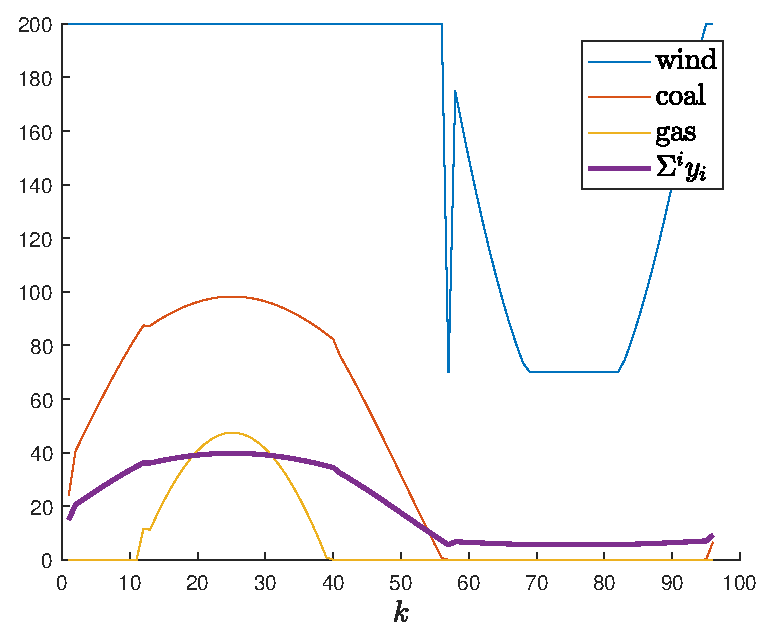
\includegraphics[width=.5\textwidth]{Figures/production.eps}
    \caption{\small Energy production per generator and market price over 24 hrs (96 quarters). Wind generators operate at maximum capacity until price is under ??. Coal plant operates when price is above ??. Gas plant only operates when price is above??. Total production vs total consumption is shown in Figure \ref{fig: supvsdem} }
  %  \label{fig: prod}
\end{figure}


\begin{figure}
    \centering
    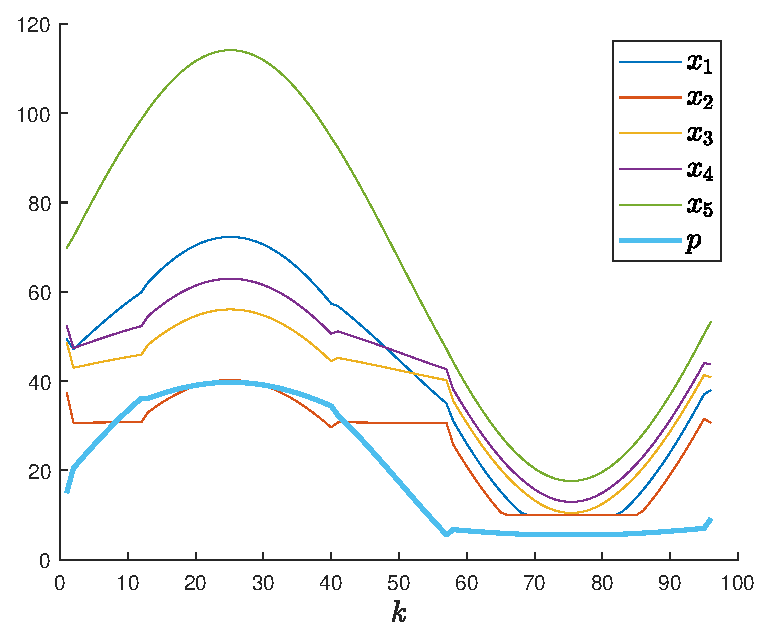
\includegraphics[width=.5\textwidth]{Figures/consumption.eps}
    \caption{\small Energy consumption per consumer and market price over 24 hrs. Consumers follow a sinusoidal desired consumption. The inelastic consumer 5 does not deviate from the desired consumption. The other consumers reduce their consumption when prices are high according to their price elasticity. }
    \label{fig: cons}
\end{figure}
\begin{figure}
    \centering
    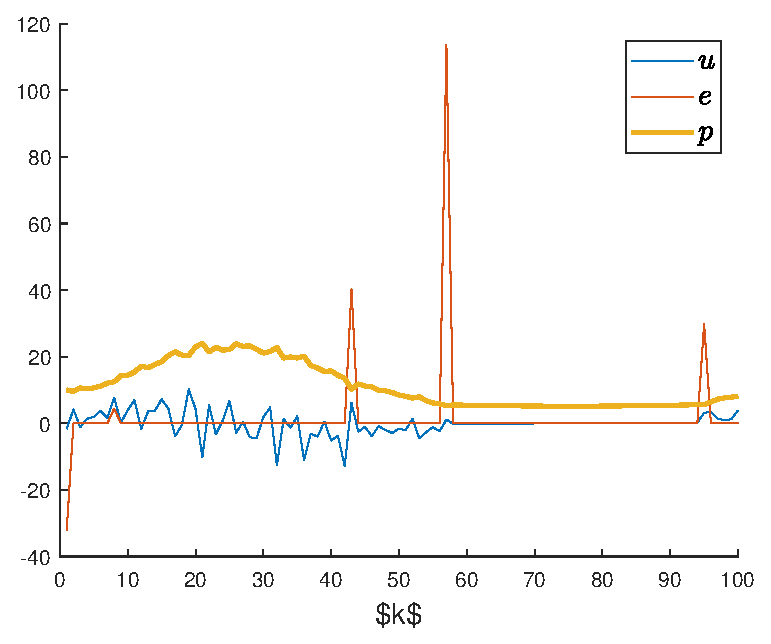
\includegraphics[width=.5\textwidth]{Figures/auctioneer.eps}
    \caption{\small Price adjustment and excess demand over 24 hours. TSO generates a price adjustment based on the excess demand. The market price is the integral of the price adjustments.}
 %   \label{fig: cont}
\end{figure}


\begin{figure}
    \centering
    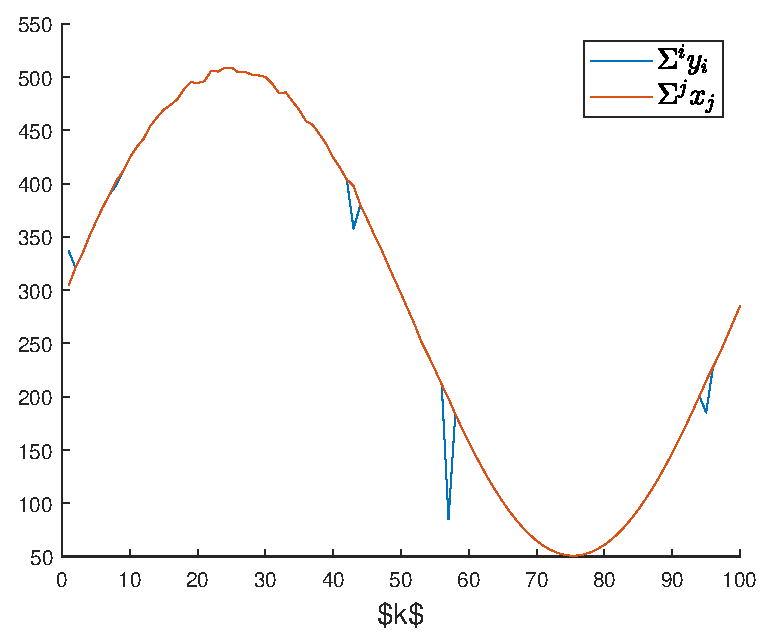
\includegraphics[width=.5\textwidth]{Figures/supvsdem.eps}
    \caption{\small Total energy supply vs total energy demand}
%    \label{fig: supvsdem}
\end{figure}

\end{comment}
\end{document}
